\documentclass{article}
\usepackage{physics}
\usepackage{graphicx}
\usepackage{caption}
\usepackage{amsmath}
\usepackage{bm}
\usepackage{framed}
\usepackage{authblk}
\usepackage{empheq}
\usepackage{amsfonts}
\usepackage{esint}
\usepackage[makeroom]{cancel}
\usepackage{dsfont}
\usepackage{centernot}
\usepackage{mathtools}
\usepackage{subcaption}
\usepackage{bigints}
\usepackage{amsthm}
\theoremstyle{definition}
\newtheorem{lemma}{Lemma}
\newtheorem{defn}{Definition}[section]
\newtheorem{prop}{Proposition}[section]
\newtheorem{rmk}{Remark}[section]
\newtheorem{thm}{Theorem}[section]
\newtheorem{exmp}{Example}[section]
\newtheorem{prob}{Problem}[section]
\newtheorem{sln}{Solution}[section]
\newtheorem*{prob*}{Problem}
\newtheorem{exer}{Exercise}[section]
\newtheorem*{exer*}{Exercise}
\newtheorem*{sln*}{Solution}
\usepackage{empheq}
\usepackage{tensor}
\usepackage{xcolor}
%\definecolor{colby}{rgb}{0.0, 0.0, 0.5}
\definecolor{MIT}{RGB}{163, 31, 52}
\usepackage[pdftex]{hyperref}
%\hypersetup{colorlinks,urlcolor=colby}
\hypersetup{colorlinks,linkcolor={MIT},citecolor={MIT},urlcolor={MIT}}  
\usepackage[left=1in,right=1in,top=1in,bottom=1in]{geometry}

\usepackage{newpxtext,newpxmath}
\newcommand*\widefbox[1]{\fbox{\hspace{2em}#1\hspace{2em}}}

\newcommand{\p}{\partial}
\newcommand{\R}{\mathbb{R}}
\newcommand{\C}{\mathbb{C}}
\newcommand{\lag}{\mathcal{L}}
\newcommand{\nn}{\nonumber}
\newcommand{\ham}{\mathcal{H}}
\newcommand{\M}{\mathcal{M}}
\newcommand{\I}{\mathcal{I}}
\newcommand{\K}{\mathcal{K}}
\newcommand{\F}{\mathcal{F}}
\newcommand{\w}{\omega}
\newcommand{\lam}{\lambda}
\newcommand{\al}{\alpha}
\newcommand{\be}{\beta}
\newcommand{\x}{\xi}

\newcommand{\G}{\mathcal{G}}

\newcommand{\f}[2]{\frac{#1}{#2}}

\newcommand{\ift}{\infty}

\newcommand{\lp}{\left(}
\newcommand{\rp}{\right)}

\newcommand{\lb}{\left[}
\newcommand{\rb}{\right]}

\newcommand{\lc}{\left\{}
\newcommand{\rc}{\right\}}


\newcommand{\V}{\mathbf{V}}
\newcommand{\U}{\mathcal{U}}
\newcommand{\Id}{\mathcal{I}}
\newcommand{\D}{\mathcal{D}}
\newcommand{\Z}{\mathcal{Z}}

%\setcounter{chapter}{-1}


\usepackage{enumitem}



\usepackage{listings}
\captionsetup[lstlisting]{margin=0cm,format=hang,font=small,format=plain,labelfont={bf,up},textfont={it}}
\renewcommand*{\lstlistingname}{Code \textcolor{violet}{\textsl{Mathematica}}}
\definecolor{gris245}{RGB}{245,245,245}
\definecolor{olive}{RGB}{50,140,50}
\definecolor{brun}{RGB}{175,100,80}

%\hypersetup{colorlinks,urlcolor=colby}
\lstset{
	tabsize=4,
	frame=single,
	language=mathematica,
	basicstyle=\scriptsize\ttfamily,
	keywordstyle=\color{black},
	backgroundcolor=\color{gris245},
	commentstyle=\color{gray},
	showstringspaces=false,
	emph={
		r1,
		r2,
		epsilon,epsilon_,
		Newton,Newton_
	},emphstyle={\color{olive}},
	emph={[2]
		L,
		CouleurCourbe,
		PotentielEffectif,
		IdCourbe,
		Courbe
	},emphstyle={[2]\color{blue}},
	emph={[3]r,r_,n,n_},emphstyle={[3]\color{magenta}}
}






\begin{document}
\begin{framed}
\noindent Name: \textbf{Huan Q. Bui}\\
Course: \textbf{8.370 - QC}\\
Problem set: \textbf{\#3}\\
Due: Wednesday, Oct 5, 2022\\
Collaborators: 
\end{framed}

\noindent \textbf{1. Find a matrix whose square is $\sigma_x$.}\\

\noindent We can easily find a matrix whose square is $\sigma_z$:
\begin{align*}
	M = \begin{pmatrix}
		1 & 0 \\ 0 & i
	\end{pmatrix}
\end{align*}
Now, since $H \sigma_z H = \sigma_x$, where $H$ is the Hadamard, consider the matrix
\begin{align*}
	N = HMH = \f{1}{2}\begin{pmatrix}
		1 & 1 \\ 1 & -1
	\end{pmatrix}
	\begin{pmatrix}
		1 & 0 \\ 0 & i
	\end{pmatrix}
	\begin{pmatrix}
		1 & 1 \\ 1 & -1
	\end{pmatrix}
	= \f{1}{2}
	\begin{pmatrix}
		1 + i & 1 - i \\ 1 -i & 1 + i
	\end{pmatrix}
\end{align*}
We find that
\begin{align*}
	N^2 = \f{1}{4}
	\begin{pmatrix}
		1 + i & 1 - i \\ 1 -i & 1 + i
	\end{pmatrix} 
\begin{pmatrix}
1 + i & 1 - i \\ 1 -i & 1 + i
\end{pmatrix} = \begin{pmatrix}
0 & 1 \\ 1 & 0 
\end{pmatrix} = \sigma_x.
\end{align*}
So $N$ is a matrix whose square is $\sigma_x$.\\



\noindent \textbf{2. Making a SWAP gate.}\\

\noindent Consider two CNOT gates where different qubits are taken as the control qubit:
\begin{align*}
	CNOT_{1} = \begin{pmatrix}
		1 & 0 & 0 & 0 \\
		0 & 1 & 0 & 0 \\
		0 & 0 & 0 & 1 \\
		0 & 0 & 1 & 0
	\end{pmatrix} \quad\quad 
	CNOT_{2} = \begin{pmatrix}
		1 & 0 & 0 & 0 \\
		0 & 0 & 0 & 1 \\
		0 & 0 & 1 & 0 \\
		0 & 1 & 0 & 0 
	\end{pmatrix}
\end{align*}
The SWAP gate is then given by 
\begin{align*}
	SWAP = CNOT_2 \cdot  CNOT_1 \cdot  CNOT_2 = \begin{pmatrix}
		1 & 0 & 0 & 0 \\
		0 & 0 & 1 & 0 \\
		0 & 1 & 0 & 0 \\
		0 & 0 & 0 & 1
	\end{pmatrix} \,\,\,\, \checkmark
\end{align*}


\noindent \textbf{3. Controlled Hadamard gate.}\\

\noindent One way to construct this gate is first SWAP 1 and 2, then apply the controlled-Hadamard on the last two qubits (with qubit 3 being the control qubit), then SWAP 1 and 2 again:
\begin{align*}
	CH_{c=3,t=1} &= SWAP_{12} CH_{c=3,t=2} SWAP_{12} = (SWAP_{12}\otimes \Id_3) (\Id_1\otimes CH_{c=3,t=2} ) (SWAP_{12}\otimes \Id_3)\\
	&= \begin{pmatrix}
		1 &0&0&0&0&0&0&0 \\
		0& 1/\sqrt{2}&0&0&0&1/\sqrt{2}&0&0 \\
		0&0&1&0&0&0&0&0 \\
		0&0&0&1/\sqrt{2}&0&0&0&1/\sqrt{2} \\ 
		0&0&0&0&1&0&0&0 \\
		0&1/\sqrt{2}&0&0&0&-1/\sqrt{2}&0&0 \\
		0&0&0&0&0&0&1&0 \\
		0&0&0&1/\sqrt{2}&0&0&0&-1/\sqrt{2} 
	\end{pmatrix}
\end{align*}
Here we have used 
\begin{align*}
	CH_{c=3,t=2} = \begin{pmatrix}
		1 & 0 & 0 & 0 \\
		0 & 1/\sqrt{2} & 0 & 1/\sqrt{2} \\
		0 & 0 & 1 & 0 \\
		0 & 1/\sqrt{2} & 0 & -1/\sqrt{2}
	\end{pmatrix}.
\end{align*}

\noindent \textbf{4. The Fredkin gate.}

\begin{enumerate}[label=(\alph*)]
	\item The Fredkin gate is a controlled SWAP gate. If $x=0$, we do nothing. If $x=1$, we swap $y$ and $z$. 
	\begin{itemize}
		\item AND gate: obtained by fixing $y_\text{in}=0$. $(x_\text{in},0,z_\text{in}) \to (x_\text{in},\text{output}, \text{junk})$. Truth table:
		\begin{align*}
			(\mathbf{0},0,\mathbf{0}) \to (0,\mathbf{0},0)\\
			(\mathbf{0},0,\mathbf{1}) \to (0,\mathbf{0},1)\\
			(\mathbf{1},0,\mathbf{0}) \to (1,\mathbf{0},0)\\
			(\mathbf{1},0,\mathbf{1}) \to (1,\mathbf{1},0)
		\end{align*}
		\item OR gate: obtained by fixing $y_\text{in}=1$. $(x_\text{in},1,z_\text{in}) \to (x_\text{in},\text{junk}, \text{output})$. Truth table:
		\begin{align*}
			(\mathbf{0},1,\mathbf{0}) \to (0,{1},\mathbf{0})\\
			(\mathbf{0},1,\mathbf{1}) \to (0,{1},\mathbf{1})\\
			(\mathbf{1},1,\mathbf{0}) \to (1,{0},\mathbf{1})\\
			(\mathbf{1},1,\mathbf{1}) \to (1,{1},\mathbf{1})
		\end{align*}
		\item NOT gate:  Fixing $y_\text{in}=1$ and $z_\text{in}=0$. $(x_\text{in},1,0) \to (\text{junk},\text{output}, \text{junk})$. Truth table:
		\begin{align*}
			(\mathbf{0},{1},{0}) \to (0,\mathbf{1},{0})\\
			(\mathbf{1},{1},{0}) \to (1,\mathbf{0},{1})
		\end{align*}
		
		\item FANOUT gate: Fixing $y_\text{in}=1$ and $z_\text{in}=0$ just like in the NOT case. Except that we use different bits for our output.  $(x_\text{in},1,0) \to (\text{output},\text{junk}, \text{output})$. Truth table:
		\begin{align*}
			(\mathbf{0},{1},{0}) \to (\mathbf{0},{1},\mathbf{0})\\
			(\mathbf{1},{1},{0}) \to (\mathbf{1},{0},\mathbf{1})
		\end{align*}
	\end{itemize}

	\item We show that the Fredkin gate preserves the number of 1s in the system by exhaustion. Truth table:
	\begin{align*}
		(0,0,0) \to (0,0,0)\\
		(0,0,1) \to (0,0,1)\\
		(0,1,0) \to (0,1,0)\\
		(0,1,1) \to (0,1,1)\\
		(1,0,0) \to (1,0,0)\\
		(1,0,1) \to (1,1,0)\\
		(1,1,0) \to (1,0,1)\\
		(1,1,1) \to (1,1,1)
	\end{align*}
	Notice that the number of 1s is preserved in all cases, as desired. 
	
	\item The half-adder is defined by 
	\begin{align*}
		(x,y) \to (x \land y, x \oplus y)
	\end{align*}
	The truth table for the half-adder is 
	\begin{align*}
		(0,0) \to (0,0) \\
		(0,1) \to (0,1) \\
		(1,0) \to (0,1) \\
		(1,1) \to (1,0) 
	\end{align*}
	Consider the following circuit using 03 Fredkin gates and 4 bits $a,b,c,d$, where $a,b$ are inputs and $c=1,d=0$ are ancillary bits. The output bits will be $(b,d)$. 
	\begin{figure}[!htb]
		\centering
		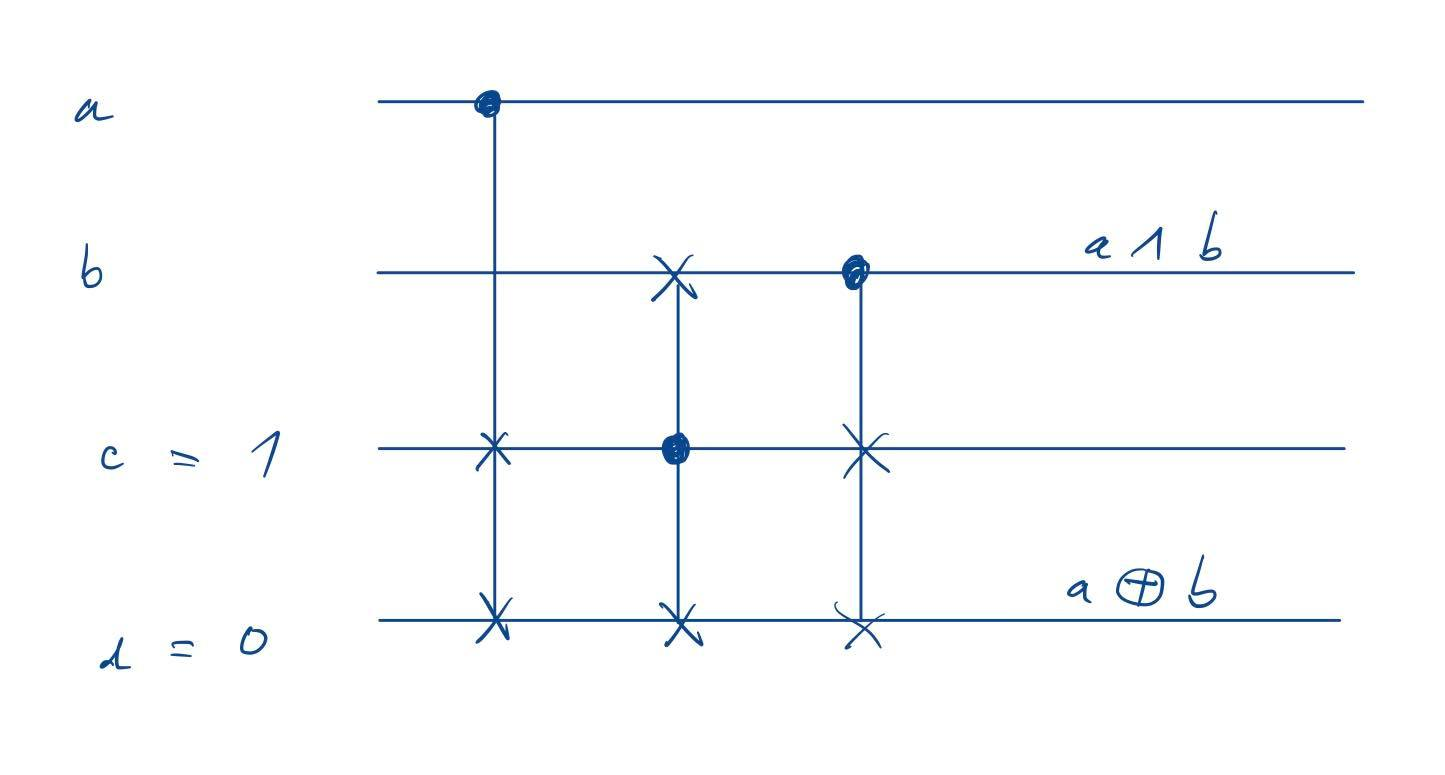
\includegraphics[scale=0.2]{fredkin.jpg}
	\end{figure}



	The circuit works as follows:
	\begin{align*}
		(a,b,c,d) = (\mathbf{0},\mathbf{0},1,0) \to (0,0,1,0) \to (0,0,1,0) \to (0,\mathbf{0},1,\mathbf{0}) \\
		(a,b,c,d) = (\mathbf{0},\mathbf{1},1,0) \to (0,1,1,0) \to (0,0,1,1) \to (0,\mathbf{0},1,\mathbf{1}) \\
		(a,b,c,d) = (\mathbf{1},\mathbf{0},1,0) \to (1,0,0,1) \to (1,0,0,1) \to (1,\mathbf{0},0,\mathbf{1}) \\
		(a,b,c,d) = (\mathbf{1},\mathbf{1},1,0) \to (1,1,0,1) \to (1,1,0,1) \to (1,\mathbf{1},1,\mathbf{0})
	\end{align*}
	
	
	
\end{enumerate}



\noindent \textbf{5. Constructing a quantum Toffoli gate.}

\begin{enumerate}[label=(\alph*)]
	\item The unitary operation the circuit implement is 
	\begin{align*}
		M 
		= H_3 \cdot  T_3 \cdot  CNOT_{13} \cdot T_3^\dagger \cdot CNOT_{23} \cdot T_3 \cdot CNOT_{13} \cdot T_3^\dagger \cdot CNOT_{23} \cdot H_3 
		= \begin{pmatrix}
			1&&&&&&& \\
			&1&&&&&& \\
			&&1&&&&& \\
			&&&1&&&& \\
			&&&&1&&& \\
			&&&&&1&& \\
			&&&&&&0&-i \\
			&&&&&&-i&0 
		\end{pmatrix}
	\end{align*}
	which is almost a Toffoli gate. The unitary transformation this circuit implements is a controlled-controlled-NOT with an extra phase shift of $e^{-i\pi/2}$. A Toffoli gate is simply a controlled-controlled-NOT, without the extra phase shift. \\

	Mathematica code:
	\begin{lstlisting}
		(*Problem 5*)
		
		H3 = KroneckerProduct[Id, KroneckerProduct[Id, HadamardMatrix[2]]];
		
		T3 = KroneckerProduct[Id, 
		KroneckerProduct[Id, {{1, 0}, {0, Exp[I*Pi/4]}}]];
		
		CNOT = {{1, 0, 0, 0}, {0, 1, 0, 0}, {0, 0, 0, 1}, {0, 0, 1, 0}};
		
		CNOT12 = KroneckerProduct[CNOT, Id];
		
		CNOT23 = KroneckerProduct[Id, CNOT];
		
		CNOT13 = KroneckerProduct[SWAP12, Id] . CNOT23 . 
		KroneckerProduct[SWAP12, Id];
		
		In[121]:= circ = 
		H3 . T3 . CNOT13 . ConjugateTranspose[T3] . CNOT23 . T3 . CNOT13 . 
		ConjugateTranspose[T3] . CNOT23 . H3
		
		Out[121]= {{1, 0, 0, 0, 0, 0, 0, 0}, {0, 1, 0, 0, 0, 0, 0, 0}, {0, 0, 
				1, 0, 0, 0, 0, 0}, {0, 0, 0, 1, 0, 0, 0, 0}, {0, 0, 0, 0, 1, 0, 0, 
				0}, {0, 0, 0, 0, 0, 1, 0, 0}, {0, 0, 0, 0, 0, 0, 0, -I}, {0, 0, 0, 
				0, 0, 0, -I, 0}}
	\end{lstlisting}

	\item To correct for the undesired phase shift, we also have to apply some sort of phase shift on the first two quantum wires as well. However, since we don't want to add the phase shift for all inputs, it has to be a controlled-phase shift gate. Consider the ansatz:
	\begin{align*}
		CP_{12}(\phi) = \begin{pmatrix}
			1 &0&0&0\\
			0&1&0&0\\
			0&0&1&0\\
			0&0&0&e^{i\phi}
		\end{pmatrix}
	\end{align*}
	Apply this before the circuit given by the problem, we find 
	\begin{align*}
		M\cdot ( CP_{12}(\phi) \otimes \mathbb{I}_3) = \begin{pmatrix}
			1&&&&&&& \\
			&1&&&&&& \\
			&&1&&&&& \\
			&&&1&&&& \\
			&&&&1&&& \\
			&&&&&1&& \\
			&&&&&&0&-ie^{i\phi} \\
			&&&&&&-i e^{i\phi}&0 
		\end{pmatrix}
	\end{align*}
	We see that to get the desired Toffoli gate, we want to set $\phi = \pi/2$. This means that we want to construct the gate
	\begin{align*}
		CP_{12}(\pi/2) = \begin{pmatrix}
			1 &0&0&0\\
			0&1&0&0\\
			0&0&1&0\\
			0&0&0&i
		\end{pmatrix}
\end{align*}
To this end, we will need CNOTs (both of them!) and the single-qubit phase gate 
\begin{align*}
	P(\theta) = \begin{pmatrix}
		1 & 0 \\ 0 & e^{i\theta}
	\end{pmatrix}
\end{align*}
We observe that $CP_{12}(\pi/2)$ is close to a controlled-$R_z(\pi/2)$, but not quite.  So, we start by decomposing $CP_{12}(\pi/2)$ as 
\begin{align*}
	CP_{12}(\pi/2) = \begin{pmatrix}
		1&&&\\
		&1&&\\
		&&e^{i\pi/4}&\\
		&&&e^{i\pi/4}
	\end{pmatrix}
\begin{pmatrix}
	1&&&\\
	&1&&\\
	&&e^{-i\pi/4}&\\
	&&&e^{i\pi/4}
\end{pmatrix} = M_1 \cdot M_2
\end{align*}
$M_2$ is simply a controlled-$R_z(\pi/2)$, which can be constructed through the procedure given in lecture
\begin{align*}
	M_2 = \mathbb{I}_1\otimes R_z(-\pi/4) \cdot CNOT_{12} \cdot \mathbb{I}_1\otimes R_z(\pi/4) \cdot CNOT_{12}
\end{align*}
where
\begin{align*}
	R_z(\theta) = \begin{pmatrix}
		e^{i\theta/2} & 0 \\ 0 & e^{-i\theta/2}
	\end{pmatrix}.
\end{align*}

$M_1$ is given by 
\begin{align*}
	M_1 &= SWAP \cdot (\mathbb{I}_1\otimes P(\pi/4)) \cdot SWAP \\
	&= CNOT_{12}\,CNOT_{21}\, CNOT_{12} \cdot \mathbb{I}_1\otimes P(\pi/4) \cdot CNOT_{12}\, CNOT_{21}\, CNOT_{12}.
\end{align*}
Here I'm following $CNOT_{12} = CNOT_1$ and $CNOT_{21} = CNOT_2$, with $CNOT_i$ defined as in Problem 2. With this, we're done. The Toffoli gate can now be constructed from the circuit provided by the problem and single qubit gates and CNOTs on the first two quantum wires:
\begin{align*}
	\text{Toff} 
	&= M\cdot ( CP_{12}(\pi/2) \otimes \mathbb{I}_3)\\
	&= M\cdot  [ (M_1\cdot M_2) \otimes \mathbb{I}_3] \\
	&= M\cdot [ (C_{12}\,C_{21}\, C_{12} \cdot \mathbb{I}_1\otimes P(\pi/4) \cdot C_{12}\, C_{21}\, C_{12}\cdot \mathbb{I}_1\otimes R_z(-\pi/4) \cdot C_{12} \cdot \mathbb{I}_1\otimes R_z(\pi/4)\cdot C_{12} ) \otimes \mathbb{I}_3]
\end{align*}
where I've abbreviated $CNOT_i$ with $C_i$.



\end{enumerate}




\end{document}











